\documentclass{article}
\usepackage[T1]{fontenc}
\usepackage{lmodern}
\usepackage{graphicx}
\usepackage{amsmath,amssymb}
\usepackage[a4paper,margin=2cm]{geometry}
\usepackage[absolute,overlay]{textpos}
\setlength{\TPHorizModule}{1mm}
\setlength{\TPVertModule}{1mm}
\usepackage[indonesian]{babel}
\usepackage{hyperref}
\setlength{\emergencystretch}{2em}
% unit: Halaman 6

\begin{document}

% === Halaman 6 (python/native) ===

6

A. Cipher Substitusi

• Contoh yang terkenal: Caesar Cipher

• Tiap huruf alfabet digeser 3 huruf ke kanan

 Plainteks :  A B C D E F G H I J K L M N O P Q R S T U V W X Y Z

 Cipherteks : D E F G H I J K L M N O P Q R S T U V W X Y Z A B C

• Contoh: 

 Plainteks: 

temui saya di jembatan merah nanti malam

 Cipherteks: 

WHPXL VDBD GL MHPEDWDQ PHUDK QDQWL PDODP

http://images.google.co.id/images?q=tbn:rVwqykNcFLzTdM:http://www.lucidcafe.com/library/96jul/96julgifs/caesar.gif

http://images.google.co.id/images?q=tbn:nJHPWFJZH0Ad0M:http://www.markchurms.com/Merchant2/graphics/caesar-d.jpg

% deskripsi: gambar native xref 52
\noindent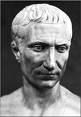
\includegraphics[width=0.85\textwidth]{../../images/python/page_006_img_01.jpeg}

% deskripsi: gambar native xref 54
\noindent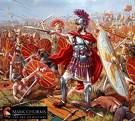
\includegraphics[width=0.85\textwidth]{../../images/python/page_006_img_02.jpeg}

% deskripsi: gambar native xref 55
\noindent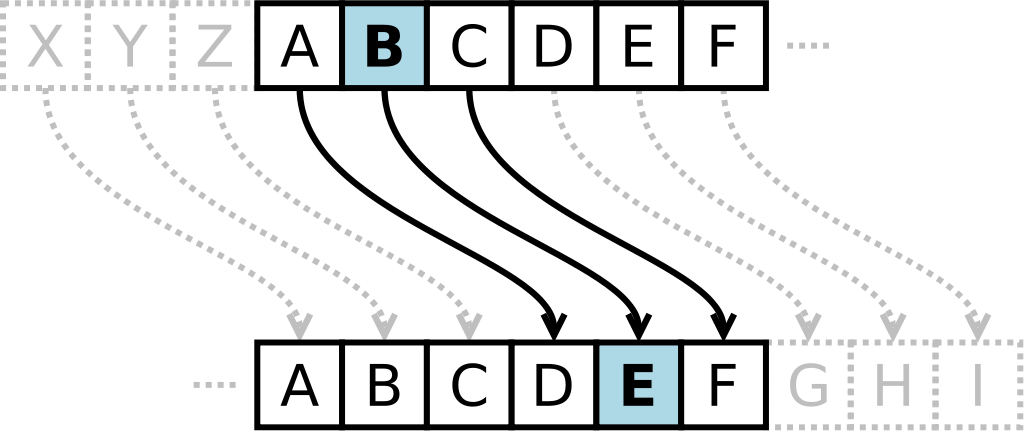
\includegraphics[width=0.85\textwidth]{../../images/python/page_006_img_03.png}

\end{document}
